\documentclass{article}
\usepackage{authblk,graphicx}
\usepackage{fancybox}% Enable the fancybox macro for landscape tables
\usepackage{multirow}

%% Caption command good for all figures, indecies, etc.
\newcommand{\mycaption}[3]{
\caption[#1]{\textsf{#2.} \label{#1} \small{\linespread{1}#3}}
}

% Draft stuff
%
%********
\def\draftversion{Y}                % Y for draft, N for final version
%********
\def\note[#1]#2{\message{(#1)}\if\draftversion
{\noindent\em[#2]\/}\fi}
%
% Mark all printed pages for draft version using dvips \specials
%
\if \draftversion Y
\special{!userdict begin /bop-hook{gsave 200 30 translate 66 rotate
  /Times-Roman findfont 160 scalefont setfont 0 0 moveto 0.85 setgray
  (Preliminary) show grestore}def end}
\fi
\def\@oddhead{
         \vbox{\hbox to\hsize{\sl \rightmark \hfill  }
              \vspace{2pt} \hbox to\hsize{\hrulefill}}}


\begin{document}
\title{ANITA-4 Flight Software Overview}
\author{R.J. Nichol}
  
%\date{April, 2003}
\date{\today}
\maketitle

%%\tableofcontents 

\section{Introduction}
During the ANITA-5 flight the ANITA flight software will be running on the flight computer acquiring and generating data. A schematic overview of the flight software processes is shown in Figure~\ref{f:overview}.

  \begin{figure}[hbt]
    \centering
    \resizebox{\textwidth}{!}{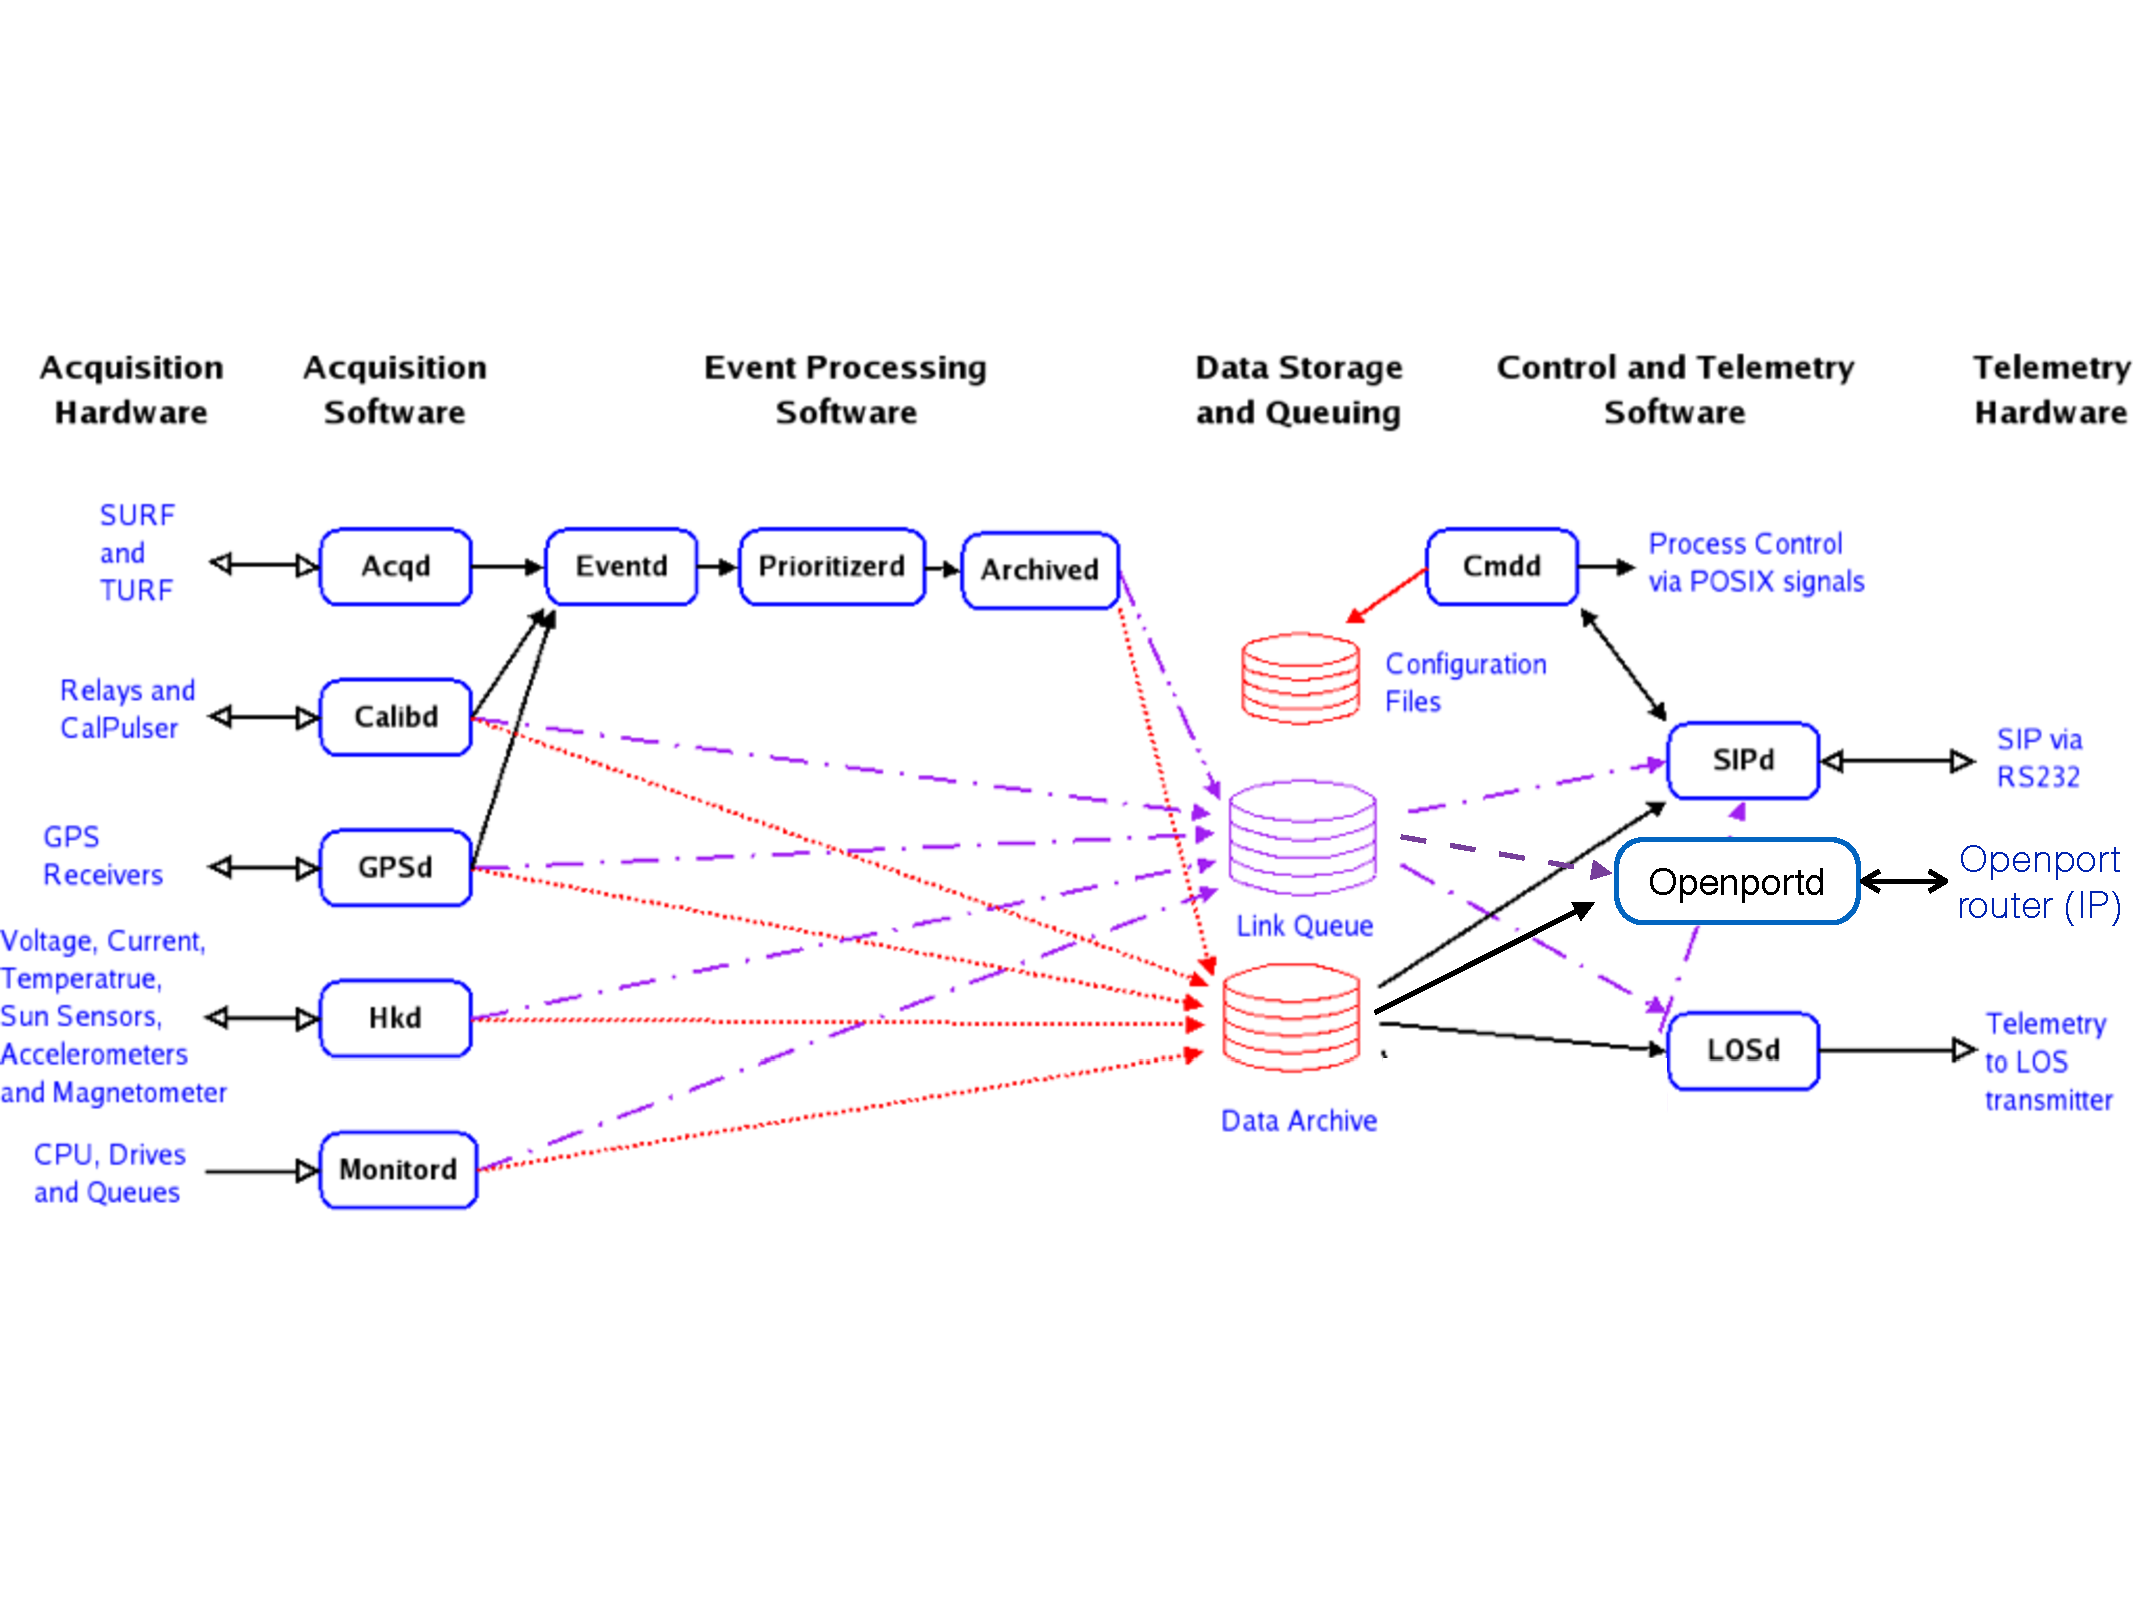
\includegraphics{fred.pdf}}
    \caption{A schematic overview of the flight software processes. The open arrows show software interaction with hardware components, and closed arrows indicate data transfer between processes. The telemetry data flow, across the ramdisk, is indicated by the dot-dashed (purple) line, and permanent data storage to the on-board drives is shown by the the dotted (red) lines.}
    \label{f:overview}    
  \end{figure}

The flight software processes break down into three main areas, which will be discussed in following sections. These areas are:
\begin{enumerate}
\item Data acquisition -- processes which control specific hardware and through which all data from that hardware is obtained.
\item Event processing -- processes which augment or analyse the waveform data in the online environment.
\item Control and telemetry -- processes which control the telemetry hardware and those which are responsible for process control.  
\end{enumerate}



\section{Data Acquisition}
The bulk of the data, around 98\%, acquired during the flight is in the form of digitized waveform data from the SURF boards. The remaining 2\% consists of auxiliary information necessary to process and interpret the waveform data (payload position, trigger thresholds, etc.) and data that is used to monitor the health of the instrument during flight (temperatures, voltages, disk spaces, etc.).

\subsection{Waveform Data}
The process that is responsible for the digitisation and triggering hardware, the SURF and TURF, is Acqd (the Acquisition Daemon). The Acqd process has four main tasks:
\begin{itemize}
\item Acquiring waveform data from the SURFs
\item Acquiring trigger and timing data from the TURF (via TURFIO).
\item Acquiring housekeeping data from the SURF (scaler rates, read back thresholds, and RF power).
\item Setting the thresholds and trigger band masks to control the trigger, dynamically adjusting the thresholds to maintain a constant rate.
\end{itemize}

Once the TURF has triggered an event and the SURFs have finished digitising, the event data is available for transfer across the c-PCI backplane to the flight computer. The flight computer polls the TURFIO to check when an event has finished digitising and the data is ready to be transferred across the c-PCI backplane. An event consists of 260 16-bit waveform data words per channel, there are 9 channels per SURF and 12 SURFs in the c-PCI crate.

\subsubsection{Trigger Control}
In addition to acquiring the waveform and trigger data, Acqd is also responsible for setting the thresholds and phi masks that control the trigger.  There are two main handles through which Acqd can control the trigger:
\begin{itemize}
\item The single channel trigger thresholds (96 channels -- 48 antennas, two polarisations.).
\item The two phi masks (H\&V).
\end{itemize}

The default mode of operation is to have all of the masks off, such that every antenna can participate in the trigger. In the thermal regime, i.e. away from anthropogenic RF noise sources such as camps and bases, the trigger control operates by dynamically adjusting the single channel thresholds to ensure that each trigger channel triggers at the same rate (typically 450kHz). The dynamic adjusting of the thresholds is necessary as even away from man-made noise sources the RF power in view varies with the temperature of the antenna and its field of view, i.e with the position of the sun and galactic centre with respect to the antenna. The thresholds are varied using a simple PID (proportional integral differential) servo loop that was tuned in the laboratory using RFCMs with terminated inputs.

When we are running in normal data taking mode, since we are servoing on them, the values of the single antenna trigger scalers should all be very similar. However, the thresholds should change as the payload rotates and the noise environment of each antenna chnages. This means that the thresholds proivde a means of tracking the noise environment of each channel, as do the RF power monitors.

During times when the balloon is in view of large noise sources, such as McMurdo station, a different triggering regime is necessary to avoid swamping the downstream processes with an unmanageable event rate. The payload automatically masks off phi sectors which are contributing too many triggers in a given time period. These are controllable via paramters in the Acqd.config which are adjustable by command.

\subsection{Housekeeping Data}
In addition to the waveform data, housekeeping data is also continuously captured, both for use in event analysis and also for monitoring the health of the instrument during flight. Table~\ref{t:housekeeping} is a summary of the various types of housekeeping data acquired by the flight software processes.

\begin{table}[hbt]
  \centering
  \begin{tabular}{| c | l | c |}
\hline
    Process & Housekeeping Data & Rate \\
\hline
Acqd & Trigger rates and average RF power & 20\,Hz \\
GPSd & GPS position, velocity, attitude, satellites, etc. & up to 5\,Hz  \\
Hkd/Calibd & Voltages, currents, temperatures, pressures, etc. & up to 5\,Hz \\
Monitord & CPU and disk drive status  & 0.03\,Hz\\
LogWatchd & Sends down config files and logs  & Each run\\
\hline
  \end{tabular}
  \caption{The types of housekeeping data acquired by flight software processes.}
  \label{t:housekeeping}
\end{table}


\section{Online Event Processing}
At altitude the bandwidth for downloading data from the payload to the ground systems is very limited, see Section~\ref{s:datadown}. In order to maximise the usage of this limited resource the events are processed online to determine the event priority and they are compressed and split into a suitable format for telemetry. 


\section{Control and Telemetry}
One critical aspect of the flight software for a balloon experiment is the control telemetry software. This software represents the only link between the experiment and the scientists on the ground. As such the software needs to be both very robust, to withstand a long flight away from human interaction, and also flexible enough to cope with unexpected failures during the flight.

\subsection{Data Downlink} \label{s:datadown}
During the flight it is critical to telemeter enough information that the scientists on the ground can determine whether the instrument is operating, and acquiring sensible data. All of this information needs to be pushed through one of three narrow (bandwidth limited) pipes to the ground. When close to the launch site the data is sent over a Line of Sight (LOS) transmitter with a maximum bit rate of 1mbps. Once over the horizon the only data links available are satellite links: i) a continuous 6\,kbps using the TDRSS satellite network; ii) upto 100\,kbps using the Openport network; and iii) a maximum of 240 bytes every 30 seconds of slow rate data using the IRDIUM and TDRSS networks. The slow rate links are only used to monitor payload health during times when the other, higher bandwidth, links are unavialble (due to satellite visibility and other issues). The Openport device is sold by the Iridium company and utilises an upgraded version of the Iriidum satellite network to transfer data at higher rates. The Openport data stream should not be confused with the slow rate iridium data stream.

There are several data streams that are telemetered, these are summarised in Table~\ref{tab:telem}. Clearly, only a tiny fraction of the total data written to disk is able to be telemetered to the ground using the satellite links.
\begin{table}[hbt]
  \centering

  \begin{tabular}{|c|c|c|c|c|}
    \hline
   Data Type & Size (bytes) & TDRSS  & Openport  & LOS  \\
    \hline 
    Header & 84 & 150 & 200 & 300 \\
    Waveform & 14,000 & 2 & 60 & 120 \\
    GPS & 64-312 & 6 & 100 & 300 \\
    Housekeeping & 292 & 6 & 60 & 60 \\
    Surf Hk. & 1236 & 2 & 20 & 50 \\
    Turf Rate & 136 & 5 & 60 & 60 \\
    CPU Monitor & 328 & 1 & 10 & 10 \\
    \hline
  \end{tabular}
  \caption{A summary of the data types, sizes and telemetry rates (in packets per minute) expected over the LOS, Openport and TDRSS downlinks.}
  \label{tab:telem}
\end{table}


\subsection{Commanding} \label{s:commanding}
During the flight it is possible to send commands from the ground to the payload over one of the three available links: line of sight, TDRSS and IRIDIUM. Commands are sent from one of two ground commanding machines:
\begin{itemize}
\item The LOS commanding machine  located in the payload hangar.
\item The TDRSS1 machine located next to the OCC (Operations Control Centre) in Palestine, Texas.
\end{itemize}
The two machines are connected via serial (RS232) cables to CSBF GSE (Ground Support Equipment) machines. Each science command can contain up to 20 bytes of information. The most common commands we are expecting to use during the ANITA-4 flight are shown in Table~\ref{tab:commands}.
\begin{table}[hbt]
  \centering

  \begin{tabular}{|c||c|c|c|}
    \hline
    Command & Name & Description  \\
    \hline 
    210 & Send Config Files & Telemeter config file  \\
    001 & Tail Messages & Telemeter the last N-lines of journalctl  \\
    003 & Start New Run & Stops processes and starts a new run \\
    011 & Journalctl Command &  N-lines of journalctl from a process \\
    131 & Kill Process & Tries to kill a process (Monitord may restart it)\\
    132 & Restart Process & Tries to restart the selected process  \\
    150-151 & TURN TUFF On/Off & Turn on/off the power to the amplites \\
    152-153 & TURN AMPA On/Off & Turn on/off the power to the AMPAs \\
    156-157 & TURN SB On/Off & Turn on/off the power to the short boards \\
    230 & ADU5 Trigger Flag & Enable/Disable ADU5 triggered events  \\
    231 & G12 Trigger Flag & Enable/Disable G12 triggered events  \\
    182 & Set G12 PPS Period & Set Period of G12 PPS  \\
    183 & Set G12 PPS Offset & Set Offset of G12 PPS  \\
    250/1 & Set PID Goal & Adjust the global single antenna trigger rate  \\
    250/8 & Set Channel Scale & Change the goal rate of an indivual antenna  \\
    \hline
  \end{tabular}
  \caption{The most common commands we are expecting to use, with a brief description of the intended command outcome.}
  \label{tab:commands}
\end{table}

Commands are executed by:
\begin{itemize}
\item Connecting to the commanding machine using ssh
\item Username:  
\item Password:
\item Changing to the cmdSend directory
\item Running ./cmdTui
\end{itemize}

Only one instance of cmdTui can be running at a time (at each loaction). A warning message will appear if a second process is started. Occasionally the network drop outs result in no version of cmdTui running but the /tmp/cmd.pid file being left behind. In these instances delete the /tmp/cmd.pid file.

The cmdSend program logs each command to the cmdlog and creates a json object for use by the AWARE monitoring program.

\end{document}
